\documentclass[../main.tex]{subfiles}

\begin{document}
    
    \chapter{Endogenous Growth Model}
        
        Technology growth $\dot A$ is \textbf{endogenous} instead of being set exogenously with $\frac{\dot A}{A} = g$ in previous models.
        
        \vspace{0.5cm}
        
        Capital $K(t)$ and effective labor $A(t)L(t)$ are production factors. Agents allocate factors between productions of output $Y(t)$ and knowledge growth $\dot A(t)$:
        \begin{align}
            Y(t)
            &= [(1-a_K) K(t)]^\alpha [A(t) (1-a_L) L(t)]^{1-\alpha},
            \quad \alpha \in [0, 1)
            \\
            \dot A(t)
            &= B [a_K K(t)]^\beta [a_L L(t)]^\gamma A(t)^\theta,
            \quad B > 0, \quad \beta, \gamma \ge 0
        \end{align}
        
        where $a_K, a_L$ are shares of capital and labor used to knowledge technology growth. $B$ is a ``shift parameter'' for knowledge production growth. $\theta$ is a productivity factor of technology growth.
        
        \vspace{0.5cm}
        
        Capital grows with savings without depreciation, and growth rate for labor (or population) remains exogenous:
        \begin{align}
            \dot K(t) = s Y(t),\quad
            \frac{\dot L(t)}{L(t)} = n \ge 0,
        \end{align}
        where $s$ is the savings rate.
        
    \section{Dynamics of Capital}
        
        Let $g_K(t) = \frac{\dot K(t)}{K(t)}$. We have that
        \begin{align}
            \dot K
            = s Y
            &=
            s (1-a_K)^\alpha (1-a_L)^{1-\alpha} K^\alpha (AL)^{1-\alpha}
            \\
            \implies
            \frac{\dot K}{K} = g_K(t)
            &= s (1-a_K)^\alpha (1-a_L)^{1-\alpha} \frac{AL}{K}^{1-\alpha}
            \\
            \implies
            \frac{\dot g_K(t)}{g_K(t)}
            &= (1-\alpha)
            \left(\frac{\dot A}{A} + \frac{\dot L}{L} - \frac{\dot K}{K} \right)
            \\
            &= (1-\alpha)
            \left(g_A(t) + n - g_K(t) \right).
        \end{align}
        
        Then on the \textbf{balanced growth path (BGP)}, constant $g_K(t)$ implies $\dot g_K(t) = 0$, then we have
        \begin{align}
            \frac{\dot g_K}{g_K} = 0
            \implies
            g_K^* = g_A^* + n.
        \end{align}
        
    
    \section{Dynamics of Knowledge}
        Let $g_A(t) = \frac{\dot A(t)}{A(t)}$. Then we have
        \begin{align}
            \frac{\dot A}{A} = g_A(t)
            &= B [a_K K(t)]^\beta [a_L L(t)]^\gamma A(t)^{\theta-1}
            \\
            \implies
            \frac{\dot g_A(t)}{g_A(t)}
            &= \beta \frac{\dot K}{K} + \gamma \frac{\dot L}{L} + (\theta - 1)\frac{\dot A}{A}
            \\
            &= \beta g_K + \gamma n + (\theta - 1) g_A.
        \end{align}
        
        Then on the BGP, constant $g_A$ implies $\dot g_A = 0$, when
        \begin{align}
            \frac{\dot g_A}{g_A} = 0
            \implies
            (1-\theta) g_A^*
            &= \beta g_K^* + \gamma n
            \\
            &= \beta (g_A^* + n) + \gamma n
            \\
            \implies
            g_A^*
            &= \frac{\beta + \gamma}{1- (\theta + \beta)} n,
            \quad
            g_K^* = \frac{(1- \theta) + \gamma}{1-(\theta + \beta)} n.
        \end{align}
        
        Capital and knowledge will always return to constant growth set by the exogenous parameters. 
    \section{Illustration of BGP}
        Assume simpler production function with only labor where $\alpha, \beta = 0$, then we have
        \begin{align}
            Y 
            &= A (1-a_L) L,
            \quad
            \dot A
            = B a_L L^\gamma A^\theta,
            \\
            \dot g_A
            &= \gamma n g_A + (\theta - 1) g_A^2,
            \quad
            \dot g_A = 0 \implies
            g_A^*
            = \frac{\gamma}{1-\theta}n,
        \end{align}
        
        Then we have that
        \begin{align}
            \frac{\partial \dot g_A}{\partial g_A}
            = \gamma n + 2 (\theta - 1) g_A,
            \quad
            \frac{\partial^2 \dot g_A}{\partial g_A^2}
            = 2 (\theta - 1)
        \end{align}
        
        \begin{figure}[ht!]
            \centering
            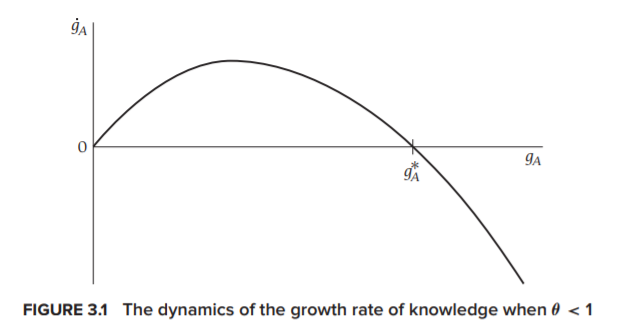
\includegraphics[width=0.5\textwidth]{subfile/attachments/3.1-dynamics-A-theta-le-0.png}
        \end{figure}
        
    
\end{document}